\documentclass[letter]{article}

\usepackage[english]{babel}
\usepackage[utf8]{inputenc}
\usepackage{amsmath}
\usepackage[colorinlistoftodos]{todonotes}
\usepackage{makecell}
\usepackage{multirow}
\usepackage{caption}
\usepackage{subcaption}
\usepackage{graphicx}
\usepackage{hyperref}
\usepackage{float}
\usepackage[all]{hypcap}
\usepackage[space]{grffile}
\usepackage{enumitem}
\usepackage{bm}
\usepackage{bbm}
\usepackage{algorithm}
\usepackage{algorithmic}
\usepackage{nccmath, mathtools}
\usepackage{amsthm,amssymb}
\usepackage{listings}

\newlist{questions}{enumerate}{1}
\setlist[questions, 1]{label = \arabic*}
\newlist{bonus}{enumerate}{1}
\setlist[bonus, 1]{label = Bonus \arabic*}

\definecolor{mygreen}{rgb}{0,0.6,0}
\definecolor{mygray}{rgb}{0.5,0.5,0.5}
\definecolor{mymauve}{rgb}{0.58,0,0.82}

\lstset{ 
	backgroundcolor=\color{white},   % choose the background color; you must add \usepackage{color} or \usepackage{xcolor}; should come as last argument
	basicstyle=\footnotesize,        % the size of the fonts that are used for the code
	breakatwhitespace=false,         % sets if automatic breaks should only happen at whitespace
	breaklines=true,                 % sets automatic line breaking
	captionpos=b,                    % sets the caption-position to bottom
	commentstyle=\color{mygreen},    % comment style
	deletekeywords={...},            % if you want to delete keywords from the given language
	escapeinside={\%*}{*)},          % if you want to add LaTeX within your code
	extendedchars=true,              % lets you use non-ASCII characters; for 8-bits encodings only, does not work with UTF-8
	frame=single,	                   % adds a frame around the code
	keepspaces=true,                 % keeps spaces in text, useful for keeping indentation of code (possibly needs columns=flexible)
	keywordstyle=\color{blue},       % keyword style
	language=Octave,                 % the language of the code
	morekeywords={*,...},            % if you want to add more keywords to the set
	numbers=left,                    % where to put the line-numbers; possible values are (none, left, right)
	numbersep=5pt,                   % how far the line-numbers are from the code
	numberstyle=\tiny\color{mygray}, % the style that is used for the line-numbers
	rulecolor=\color{black},         % if not set, the frame-color may be changed on line-breaks within not-black text (e.g. comments (green here))
	showspaces=false,                % show spaces everywhere adding particular underscores; it overrides 'showstringspaces'
	showstringspaces=false,          % underline spaces within strings only
	showtabs=false,                  % show tabs within strings adding particular underscores
	stepnumber=2,                    % the step between two line-numbers. If it's 1, each line will be numbered
	stringstyle=\color{mymauve},     % string literal style
	tabsize=2,	                   % sets default tabsize to 2 spaces
	title=\lstname                   % show the filename of files included with \lstinputlisting; also try caption instead of title
}

% Adjust margins
\addtolength{\oddsidemargin}{-0.75in}
\addtolength{\evensidemargin}{-0.75in}
\addtolength{\textwidth}{1.5in}
\addtolength{\topmargin}{-.5in}
\addtolength{\textheight}{1.5in}
\setlength\parindent{0pt}
\setlength{\parskip}{5pt}

\title{CS 520: Assignment 3 - Probabilistic Search (and Destroy)}
\author{Haoyang Zhang, Han Wu, Shengjie Li, Zhichao Xu}
\date{\today}

\begin{document}
\maketitle

\section{Introduction, group members and division of workload}
\label{sec:Introduction}

In this group project, we implemented a well-working solver that contains 5 searching strategies. This solver is also capable of dealing with a not-teleportable agent and a moving target. Our program also has a gorgeous GUI and can visualize the progress of solving by animation. \\
\begin{tabular}{| p{2.5cm} | p{\textwidth -3.5cm} |}
	\hline
	\makecell[c]{Name \\ RUID} & Workload \\
	\hline
	\makecell[c]{Haoyang Zhang \\ 188008687} & {Implemented the searching solver. Wrote UpdateExplanation.html and RuleExplanation.html which are two documents about our algorithm, covering scores of important parts of our report (We put most of them into our report). Ran test for a moving target part.} \\
	\hline
	\makecell[c]{Han Wu \\ 189008460} & {Wrote the scripts to test the algorithm for question 4 in part one and moving target part. Ran tests together with Haoyang Zhang in moving target part. Generated most of the figures in the test. Wrote part of the report about question 4 in part one and the moving target part. Wrote answer for question 5.} \\
	\hline
	\makecell[c]{Shengjie Li \\ 188008047} & {Designed and implemented the GUI of our program. Implemented a function that can generate animation of the progress of searching and destroying. Finished the format design of the report using \LaTeX. } \\
	\hline
	\makecell[c]{Zhichao Xu \\ 188008912} & {Helped revise and improve the codes through early-stage testing. Wrote scripts for experiments, did visualization and answered question 3.} \\
	\hline
\end{tabular}


\section{A Stationary Target}
\label{sec:A Stationary Target}
\subsection{Theory}
\label{sec:1-theory}
\subsubsection{Questions}
\label{sec:1-1-questions}
\begin{enumerate}
	\item {Given observations up to time $ t $ (Observations$ _t $), and a failure searching Cell$ _j $ (Observations$ _t+1 $ = Observations$_t \wedge $ Failure in Cell$ _j $), how can Bayes' theorem be used to efficiently update the belief state, i.e., compute: } 
	\begin{align}
		\mathbb{P} \text{(Target in Cell$ _i | $Observations$_t $  $\wedge $ Failure in Cell$ _j $).}
	\end{align}
	\begin{align}
		\shortintertext{When $ i \ne j $,} 
		&\mathbb{P} \text{(Target in Cell$ _i | $Observations$_t $  $\wedge $ Failure in Cell$ _j $)} \nonumber \\
		&= \alpha \mathbb{P} \text{(Target in Cell$ _i | $Observations$_t $)}. \label{eq:2} \\
		\shortintertext{Denote $ \mathbb{P} $ (Target in Cell$ _i | $Observations$_t $) by $ a_{it} $, }
		(\ref{eq:2}) &= \alpha \cdot a_{it} \nonumber. 
		\shortintertext{When $ i = j $,} 
		& \mathbb{P} \text{(Target in Cell$ _j | $Observations$_t $  $\wedge $ Failure in Cell$ _j $)} \nonumber \\
		&= \alpha \mathbb{P} \text{(Target in Cell$ _j | $Observations$_t $)}  \cdot \mathbb{P} \text{(Target not found in Cell$ _j | $Target in Cell$ _j $).} \label{eq:3} \\
		\shortintertext{Denote $ \mathbb{P} $ (Target not found in Cell$ _j | $Target in Cell$ _j $) by $ q_j $, }
		(\ref{eq:3}) &= \alpha \cdot a_{jt} \cdot q_j. \nonumber \\
		\alpha &= \frac{1}{\sum_{i \ne j} (\alpha \cdot a_{it}) + \alpha \cdot a_{jt} \cdot q_j} = \frac{1}{1 - a_{jt}(1-q_j)}. \nonumber \\
		a_{i0} &= \frac{1}{2500} \text{ for } i = 0, \dots, 2499  \nonumber
	\end{align}
	\item {Given the observations up to time $ t $, the belief state captures the \textbf{current probability the target is in a given cell}. What is the probability that the target will be \textbf{found} in Cell$ _i $ if it is searched:} 
	\begin{align}
	\mathbb{P} \text{(Target found in Cell$ _i | $Observations$_t $)?}
	\end{align}
	\begin{align*}
		&\mathbb{P} \text{(Target found in Cell$ _i | $Observations$_t $)} \\
		&= \mathbb{P} \text{(Target in Cell$ _i | $Observations$_t $)}(1-\mathbb{P} \text{(Target not found in Cell$ _i | $Target in Cell$ _i$)}) \\
		&= a_{it} \cdot (1 - q_i) \\
		a_{i0} &= \frac{1}{2500} \text{ for } i = 0, \dots, 2499 
	\end{align*}
	
\end{enumerate}

\subsubsection{Strategies of updating}
\label{sec:1-1-Strategies of updating}
\begin{enumerate}
	\item {Update search results} \\
	For a given block, there are 2 different search results: `True'(find the target) and `False'(Target not found). If the result is `True', this board is done. If the result is `False', we have to update the `prob' to represent this result.
	
	Using the notion of particle filter, assuming that each block have $N \cdot p_i$ samples. If we have not found a target in $block_k$, some samples should be cast off, i.e. $p_k' = p_k(1-q_k)$. Then, resample all blocks by multiplying $\alpha$, where $\alpha = \frac{1}{1-p_kq_k}$.
	
	In a nutshell, after searching $block_k$: 
	$p_i' = \frac{\alpha N \cdot p_i}{N}$, where $i\ne k$; 
	$p_k' = \frac{\alpha N \cdot p_k(1-q_k)}{N}$,
	$\alpha = \frac{1}{1-p_kq_k}$
	
	The pseudo code is as follows:
	\begin{algorithm}[H]
		\caption{updateP(pos)}
		\begin{algorithmic}
			\STATE prob[pos] = prob[pos] * failP[cell[pos]]
			\STATE normalize(prob)
			\RETURN 
		\end{algorithmic}
	\end{algorithm}
	\begin{algorithm}[H]
		\caption{normalize(prob)}
		\begin{algorithmic}
			\STATE normalize(prob):
			\STATE sumP = sum(prob)
			\STATE prob = prob / sumP
			\RETURN 
		\end{algorithmic}
	\end{algorithm}
	
	\item {Update with additional observations} \\
	Using the notion of particle filter, we can update reports easily. For a given cell, if it is not a possible previous block, all its samples should be ruled out. If it is a possible previous block, and if there are some possible neighbors according to the reports, its samples will migrate to them. But if there are no possible neighbors, all its samples will also be trapped in this block and die out. Then, resample all blocks.
	
	Yet, notice that reports are related to each other. For example, 2 consecutive reports H-F, C-H tell far more than ``the target first move from Hilly to Flat or from Flat to Hilly, and then move form Cave to Hilly or from Hilly to Cave''. We know that the target must move from Flat to Hilly and then to Cave.
	
	Therefore, we should consider each consecutive pair of reports and try to figure out the real moving direction. Once we know the real direction, we can pin down the direction of future reports, but also all previous reports.
	
	Notice that if we know the real direction of previous reports, we should re-filter all previous observations because observations have become more accurate.
	
	The pseudo code is as follows:
	\begin{algorithm}[H]
		\caption{updateR(report)}
		\begin{algorithmic}
			\STATE{reUpFlag, directions = solveReprot(report)}
			\IF{reUpFlag}
			\STATE{reUpdateReport(searchHistory, targetHistory)}
			\ELSE
			\STATE{updateReport(directions)}
			\ENDIF
			\RETURN
		\end{algorithmic}
	\end{algorithm}
	\begin{algorithm}[H]
		\caption{solveReport(report)}
		\begin{algorithmic}
			\IF{reportSolved}
			\STATE {direction = trackTarget(report, targetHistory[-1])}
			\STATE reUpFlag = False
			\ELSE
			\STATE {common = findCommon(report, reportHistory[-1])}
			\IF{len(common) == 1} 
			\STATE{backtrack(common, reportHistory)}
			\STATE{direction = tarckTarget(report, targetHistory[-1])}
			\STATE{reUpFlag = True}
			\ELSE
			\STATE{direction = (report, report.reverse())}
			\STATE{reUpFlag = False}
			\ENDIF
			\ENDIF
			\STATE reportHistory.append(report)
			\RETURN reUpFlag, direction
		\end{algorithmic}
	\end{algorithm}
	\begin{algorithm}[H]
		\caption{reUpdateReprot(searchHistory, targetHistory)}
		\begin{algorithmic}
			\FOR{i in range(len(searchHistory))}
			\STATE updateP(searchHistory[i])
			\STATE updateReport(((targetHistory[i], targetHistory[i+1]), ))
			\ENDFOR
			\RETURN 
		\end{algorithmic}
	\end{algorithm}
	\begin{algorithm}[H]
		\caption{updateReprot(directions)}
		\begin{algorithmic}
			\STATE{tempProb = zeros\_like(prob)}
			\FOR{prev, post in directions}
			\FOR{each block pos}
			\IF{cell[pos] == prev}
			\STATE{nPosList = where(border[pos, post])}
			\STATE{factor = len(nPosList)}
			\IF{factor}
			\FOR{each nPos in nPosList}
			\STATE{tempPorb[nPos] = tempPorb[nPos] + prob[pos] / factor}
			\ENDFOR
			\ENDIF
			\ENDIF
			\ENDFOR
			\ENDFOR
			\STATE{prob = normalize(tempProb)}
			\RETURN 
		\end{algorithmic}
	\end{algorithm}
	\begin{algorithm}[H]
		\caption{trackTarget(report, prev)}
		\begin{algorithmic}
			\STATE post = report - prev
			\STATE targetHistory.append(post)
			\RETURN post
		\end{algorithmic}
	\end{algorithm}
	\begin{algorithm}[H]
		\caption{backtrack(post, reportHistory)}
		\begin{algorithmic}
			\STATE targetHisory.insert(0, post)
			\FOR{report in reportHistory.reverse()}
			\STATE prev = reprot - post
			\STATE targetHistory.insert(0, prev)
			\ENDFOR
			\RETURN 
		\end{algorithmic}
	\end{algorithm}
\end{enumerate}

\subsubsection{Our understandings and interpretations of rules}
Denote $P(target\,\, in \,\, block_i|Observation_t)$ by $p_i$. \\
Denote $P(find\,\, the\,\, target\,\, in\,\, block_i|target\,\, is\,\, in\,\, block_i)$ by $q_i$.
\begin{enumerate}
	\item {Rule 1} \\
	A given rule in Assignment Description.
	\begin{itemize}
		\item {idea} \\
		At any time, search the cell with the highest probability of containing the target.
		\item {Implementation} \\
		$next = \arg\max\limits_i p_i$
		\item {Pseudo Code} 
		\begin{lstlisting}
maxProb():
	value = prob
	return argmax(value)
		\end{lstlisting}
	\end{itemize}
	
	\item {Rule 2} \\
	A given rule in Assignment Description.
	\begin{itemize}
		\item {idea} \\
		At any time, search the cell with the highest probability of finding the target.
		\item {Implementation} \\
		$next = \arg\max\limits_i p_iq_i$
		\item {Pseudo Code} 
		\begin{lstlisting}
maxSucP():
	value = prob * sucP
	return argmax(value)   
		\end{lstlisting}
	\end{itemize}

	\item {Rule 3} \\
	A rule just for fun.
	\begin{itemize}
		\item {idea} \\
		At any time, search the block which provides the largest information entropy
		\item {Implementation} \\
		$H_i = -(p_iq_i)log(p_iq_i)$ $next = \arg\max\limits_i H_i$
		\item {Pseudo Code} 
		\begin{lstlisting}
maxInfo():
	find = prob * sucP
	value = find * log2(find)
	return argmin(find)
		\end{lstlisting}
		\item {Discussion} \\
		Notice that $H(x)$ is increasing function in $[0, 0.5]$. If there are a large number of blocks, Rule 3 is equivalent to Rule 2.
	\end{itemize}
\end{enumerate}

\subsubsection{Some other thoughts -- double check}
\begin{itemize}
	\item {Idea} 
	\par{Notices that sometimes we might fail to find the target in Flat. Once we failed, this block’s probablity will dramatically decrease, which leads to thousands of more searching.}
	
	\par{For example, ignoring the $\alpha$, once we failed in a Flat, say $block_i$, $p_i = \frac{1}{25000}$, $p_iq_i = \frac{9}{250000} = 0.000036$. In order to search this block again, we have to make $p_jq_j < p_iq_i, j \ne i$. Therefore, we have to search other Flat blocks once, Hilly 2 times, Jungle 26 times and Cave 76 times, which is about 40 thousand times in total.}
	
	\par{Therefore, we could use double check once a block’s probability becomes too small.}
	\item {Pseudo Code} 
	\begin{lstlisting}
doubleThreshold = ceil(np.log(0.01) / log(failP) - 1

for each time search a block pos:
	doubleCounter[pos] ++
	if doubleCounter[pos] >= doubleThreshold[pos]
		update()
		search(pos)
	update()
	\end{lstlisting}
	\item {Discussion} 
	\begin{enumerate}
		\item {Even with double check, we still might fail in a Flat, which leads to a much more than 40 thousand steps search. It is, however, much unlikely to happen. According to our experiment, only about 0.4\% boards need more than 100K steps to solve.}
		\item {With double check, the number of boards need more than 100K steps are approximate to the number of more than 1M steps. But 1M steps is unacceptable, and therefore we stop solving these board and regard them as ``unsolvable''.}
		\item {Note that not only Flat, but also all blocks can apply double-check. In practice, we double check Flat and Hilly because they are the most common cases which lead to 1M steps.}
	\end{enumerate}
\end{itemize}

\subsection{Practice}
\label{sec:1-practice}
\subsubsection{Questions}
\label{sec:1-2-questions}
\begin{enumerate}
	
	\item {Consider comparing the following two decision rules:
		\begin{itemize}
			\item {Rule 1: At any time, search the cell with the highest probability of containing the target.}
			\item {Rule 2: At any time, search the cell with the highest probability of finding the target.}
		\end{itemize} 
		\par{For either rule, in the case of ties between cells, consider breaking ties arbitrarily. How can these rules be interpreted / implemented in terms of the known probabilities and belief states?}
		\par{For a fixed map, consider repeatedly using each rule to locate the target (replacing the target at a new,
			uniformly chosen location each time it is discovered). On average, which performs better (i.e., requires less
			searches), Rule 1 or Rule 2? Why do you think that is? Does that hold across multiple maps?}
		} \\
	
	\par{For a fixed map, we repeatedly used Rule 1 and Rule 2 to locate the target. The result is shown in Fig \ref{fig:xzc1}.}
	
	\begin{figure}
		\centering
		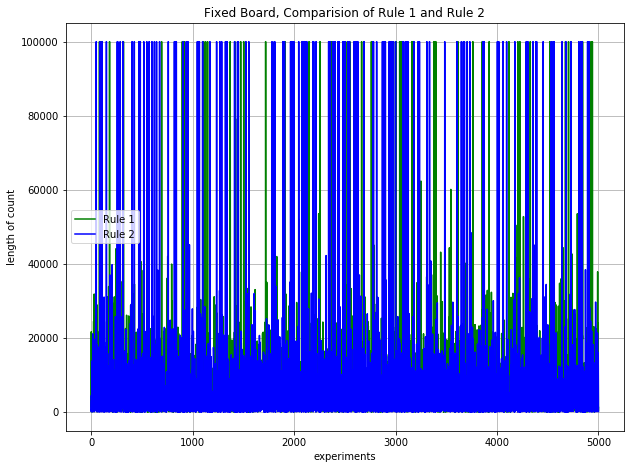
\includegraphics[width=0.7\textwidth]{fig/xzc1.png}
		\caption{Fixed Board, Comparison of Rule 1 and Rule 2}
		\label{fig:xzc1}
	\end{figure}
	
	\par{The mean and variance of Rule 1 are 6004.0966 and 56320634.4832, and the mean and variance of Rule 2 are 4539.7006 and 37546839.3709 (after eliminating the
	unsolvable cases). The fail rate for Rule 1 and Rule 2 are 0.33\% and 0.66\%. These
	numbers are calculated through 5000 times of experiments. When the number of search
	actions exceeds 100000, we note the board as unsolvable. Through our comparison, we
	came into conclusion that Rule 2 is better than Rule 1. Also, it has larger fluctuations due
	to the presence of unsolvable cases.}
	\par{According to our understanding, Rule 2 is more close to the problem itself, because we
	have $ \mathbb{P}(\text{Target not found in Cell} | \text{Target is in Cell}) $. The improvement of Rule 2 compared to Rule 1 is that Rule 2 gets rid of the conditional probability and make more accurate inferences.}
	\par{For multiple maps, such pattern still holds. The result is showed in Fig \ref{fig:xzc2}.}
	
	\begin{figure}
		\centering
		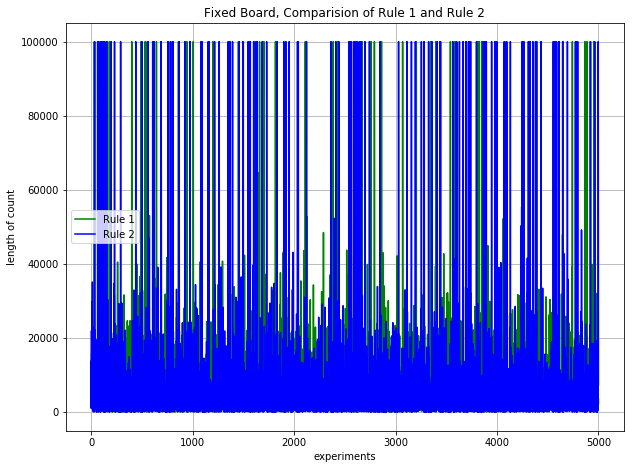
\includegraphics[width=0.7\textwidth]{fig/xzc2.png}
		\caption{Fixed Board, Comparison of Rule 1 and Rule 2}
		\label{fig:xzc2}
	\end{figure}
	
	\par{The mean and variance of Rule 1 are 6221.3866 and 59873979.75314046,
	and the mean and variance of Rule 2 are 4682.4286, 40237182.382102035 (after eliminating the unsolvable cases). The fail rate for Rule 1 and Rule 2 are 0.33\% and 0.66\%. These numbers are also calculated through 5000 times of experiments.}
	
	In addition, we used a technique what we called ``double check'' to help searching. When we move to a flat cell, we would search it again if we have failed to find the target at the first search attempt. When we move to a hilly cell, if we have failed three search attempts on this cell, we would search it again. We call this ``Double-check search'' case. We use Rule 1, Rule 2, and Rule 3 to supervise our search. Rule 1 and Rule 2 is just the ones mentioned in the context. Even though Rule 3 does not have improvement, we also do some experiments because we find it interesting. In the experiment, 5000 maps are generated and we used 3 rules to search the target in the map. The result is shown in Fig \ref{fig:part1-q345.png}.
	
	\begin{figure}[H]
		\centering
		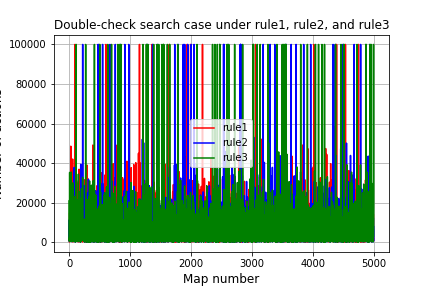
\includegraphics[width=0.7\textwidth]{fig/part1-q345.png}
		\caption{Number of actions in double-check search case}
		\label{fig:part1-q345.png}
	\end{figure}
	
	
	From the figure above, we can see that the performance of Rule 1 is the worst. Rule 2
	and Rule 3 are similar. The means of Rule1, Rule 2, and Rule 3 are 6287.49, 5223.53,
	and 5145.19. The average number of actions of Rule 2 and Rule 3 are superior to Rule 1. So, Rule 2 and Rule 3 are better in this case. The variances of Rule1, Rule 2, and Rule 3 are 54138591.92, 42819190.19, and 39314588.23. From this perspective, we can also conclude that Rule 2 and Rule 3 are better. If the number of search actions is beyond 100,000, we call it unsolvable because it is extremely hard to find the target under this circumstance. The reason of it being unsolvable is that, if the target is on a `Flat' cell or a `Hilly' cell and we have failed several times searching on that cell, we would hardly be able to find the target in a reasonable time. To avoid the waste of time, we decided to terminate the program if the number of search action is greater than 100,000, which we call it unsolvable. The fail rate of Rule1, Rule 2, and Rule 3 are 0.0026, 0.008, 0.0116. Rule 3 may sometimes not be able to find the target although it performs better.
	
	\item {Consider modifying the problem in the following way: at any time, you may only search the cell at your
		current location, or move to a neighboring cell (up/down, left/right). Search or motion each constitute a single
		`action'. In this case, the `best' cell to search by the previous rules may be out of reach, and require travel.
		One possibility is to simply move to the cell indicated by the previous rules and search it, but this may incur a
		large cost in terms of required travel. How can you use the belief state and your current location to determine
		whether to search or move (and where to move), and minimize the total number of actions required? Derive a
		decision rule based on the current belief state and current location, and compare its performance to the rule
		of simply always traveling to the next cell indicated by \textbf{Rule 1} or \textbf{Rule 2}. Discuss.} \\
	
	In this question, we need to move to the cell that we want to search and motion also
	counted as one step. We call this ``search and motion case''. We use 3 rules to guide our
	search. Rule 1 means just traveling to the ``best'' cell which is indicated by the original
	Rule 1. Rule 2 is the same case. Rule 4 is invented by ourselves. It uses new criterion to
	supervise our search. We generate 5000 maps and use different rules to search the
	target in the maps. The result is shown in Fig \ref{fig:q4}.
	
	\begin{figure}[H]
		\centering
		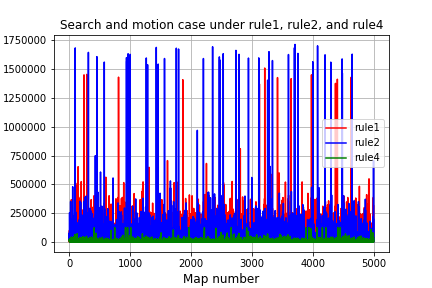
\includegraphics[width=0.7\textwidth]{fig/part1-q4.png}
		\caption{Number of actions in search and motion case}
		\label{fig:q4}
	\end{figure}
	
	From the figure, we can see that the performance of Rule 4 is better than Rule 1 and
	Rule 2. The means of Rule1, Rule 2, and Rule 4 are 58475.71, 45925.69, and 9745.66. It
	is easy to find that the average number of actions of Rule 4 is much smaller than Rule 1
	and Rule 2. The variances of Rule1, Rule 2, and Rule 4 are 7920337425.95,
	5069004957.26, and 119653468.99. From this view, we can also conclude that Rule 4 is
	better. When the number of search actions is beyond 100000, we call it unsolvable
	because it is extremely hard to find the target under this circumstance. The fail rate of
	Rule1, Rule 2, and Rule 4 are 0.0026, 0.0076, and 0.003. Rule 4 also performs well.
	
	
	\item {An old joke goes something like the following: 
		\begin{center}
			\textit{A policeman sees a drunk man searching for something under a streetlight and asks what the drunk has lost.
				He says he lost his keys and they both look under the streetlight together. After a few minutes the policeman
				asks if he is sure he lost them here, and the drunk replies, no, and that he lost them in the park. The
				policeman asks why he is searching here, and the drunk replies, ''the light is better here''.}
		\end{center}
		\par{In light of the results of this project, discuss.}
		} \\
	
	\par{There are some links between the joke and our problem. There are also some differences between the drunk man in the joke and our search policy. Streetlight is a good thing. When you have streetlight, it is easier for you to find the keys than other area if they are actually under the streetlight. Flat area is just like the streetlight in the map. When the target is in one cell, you have the highest probability to find it if the cell is flat. So, you should search the flat area at first (and the result is: Rule 2 is better than Rule 1). However, searching the flat area is just one part of our policy. Another part is that we continuously update the probability. We continuously update our knowledge about the map. And this distinguishes our policy from the drunk man’s. We update the probability of finding the target in one cell every time after we finish one search. And we search the cell with the highest probability of finding the target at the next time. When the flat cell has been searched, the probability of finding the target in the cell becomes very low. So, next time we will not choose to search it. However, the drunk man doesn’t update his knowledge about the whole area. If he didn’t find the keys under the streetlight, he should update his knowledge and go to other areas to search. It’s unwise for him to keep searching under the streetlight.} 
	\par{Another problem of the drunk man is that he doesn’t use his prior knowledge about the lost place. He remembers that he lost the keys in the park. So, he should search in the park at first although there may be no light. Actually, the drunk man’s situation is better than us. In the map, every cell has the same probability of owning the target and we know nothing about the position of the target at first.}
	
\end{enumerate}

\section{A Moving Target}
\label{sec:A Moving Target}
\par{In this section, the target is no longer stationary, and can move between neighboring cells. Each time you perform
	a search, if you fail to find the target the target will move to a neighboring cell (with uniform probability for each).
	However, all is not lost - whenever the target moves, surveillance reports to you that the target was seen at a \textbf{Type1
	$ \times $ Type2} border where Type1 and Type2 are the cell types the target is moving between (though it is not reported
	which one was the exit point and which one the entry point. }
\subsection{Theory}
\label{sec:2-theory}
\subsubsection{Optimal Rule for 1 Step in Theory}
\begin{enumerate}
	\item {Agents can teleport} \\
	For a given cell, if the target is in this cell, the expectation of search times is:
	$E(block_i) = \frac{1}{q_i}$
	For the whole board, the expectation of search times is:
	$C = E(E(block)) = \sum\limits_i\frac{p_i}{q_i} = \sum\limits_{j \ne i}\frac{p_j}{q_j} + \frac{p_i}{q_i}$
	
	If we decided to search $block_i$, by updating probabilities: (Details are in UpdateExplanation.html.)
	$C_i' = -(p_iq_iC_i+ (1-p_iq_i)0) = -p_iq_i(\sum\limits_{j \ne i}\frac{\alpha p_j}{q_j} + \frac{\alpha p_i(1-q_i)}{q_i})$, where $\alpha = \frac{1}{1-p_iq_i}$
	
	$C_i' = -\alpha p_iq_i(\sum\limits_{j \ne i}\frac{p_j}{q_j} + \frac{p_i}{q_i} - p_i) = -\alpha p_iq_i(C-p_i)$
	
	Notice that $\alpha p_iq_i = \frac{p_iq_i}{1-p_iq_i} =\alpha-1$:
	$C_i' = -(\alpha - 1)(C-p_i)$
	\item {Agents have to move step by step} \\
	In this case, we have to consider additional moving cost.
	Denote $L = C + M$, where $L$ is the total cost of a given board, $C$ is previous searching cost, and $M$ is moving Cost.
	
	If we decided to search $block_i$ from $block_k$:
	$L_i' = -p_iq_i(C_i - \sum\limits_{j \ne i}p_jd_{ij} -\alpha p_i(1-q_i)d_{ii}) - (1-p_iq_i)0 - d_{ki}$, where $d_{ij}$ is the distace from$block_i$ to $block_j$.
	
	Notice that $d_{ii} = 0$, $\alpha p_i(1-q_i)d_{ii} = 0 = \alpha p_iq_id_{ii}$
	$L_i' = -(\alpha - 1)(C - p_i - \sum\limits_j p_jd_{ij}) - d_{ki}$.
	
	Actually, case 1 is a special case of case 2 where all $d_{ij} = 0$.
\end{enumerate}
\subsubsection{Our understandings and interpretations of rules}
\begin{enumerate}
	\item {Rule 4} \\
	A rule for the case agents cannot teleport but targets are stationary.
	\begin{itemize}
		\item {idea} \\
		Since there are many blocks, $\alpha \approx 1$, and therefore $d_{ki}$ is dominant. That is to say, the best rule is actually the least moving rule. We can approximately consider that the "value" of a target decreases exponentially in term of distance.
		\item {Implementation} \\
		$next = \arg\max\limits_i \frac{p_iq_i}{2^{d_i}}$
		\item {Pseudo Code} 
		\begin{lstlisting}
minMove(pos):
	value = prob * sucP / exp2(dist[pos])
	return argmax(value)
		\end{lstlisting}
		\item {Discussion} 
		\begin{enumerate}
			\item {In order to achive the minimum moving, Here seems another rule, which seems a little bit weird: For each cell, search it a number times, then move to its unsearched neighbor. The number of each searching of a given block can be define below: \\
			$N = \lceil\frac{1}{q_i}\rceil$, which is the expectation of searching times\\
			In this case, $N(flat) = 2, N(hilly) = 2, N(Forest) = 4, N(Cave) = 10$.\\ Once we have not found the target in one round, make a U-turn and re-search all blocks in reversed order.\\
			Therefore, for a given board, $E = (\sum\limits_i (p_iN_i) + 2500)/2 = 6500$}
			\item {We cannot use Rule 5 directly because $\alpha \approx 1$. Even use float64 we still cannot distinguish some blocks.}
		\end{enumerate}
	\end{itemize}
	
	\item {Rule 5} \\
	A rule for the case agents cannot teleport and targets can move.
	\begin{itemize}
		\item {idea} \\
		In this case, many blocks are rule out becasue of witness reports. Therefore, we can directly use ``Optimal Rule'' to solve this case.
		\item {Implementation} \\
		$next = \arg\min\limits_i L_i'$
		\item {Pseudo Code} 
		\begin{lstlisting}
minCost(pos):
	factor = 1 / (1 - prob * sucP)
	base = prob / sucP
	sCost = (factor - 1) * (base - prob)
	for each block pos:
		mCost[tPos] = (factor[tPos] - 1) * sum(prob * dist[tPos])
	value = sCost - mCost - dist[pos]
	return argmax(value)  
		\end{lstlisting}
		\item {Discussion} \\
		Actually, we can show that Rule 2 is a good approximate of Rule 5 in the case hunter can teleport but target can also move. In reports, we performed an experiment to compare Rule 2 and Rule 5, and the result of them are similar.
	\end{itemize}
\end{enumerate}
	
\subsection{Practice}
\label{2-2practice}
\subsubsection{Questions}
\label{2-2-1questions}
\par{Implement this functionality in your code. How can you update your search to make use of this extra information?
	How does your belief state change with these additional observations? Update your search accordingly, and again
	compare \textbf{Rule 1} and \textbf{Rule 2}.}

	The strategies of updating is in section \ref{sec:1-1-Strategies of updating}.

\par{Re-do question 4) above in this new environment with the moving target and extra information.}

	In this problem, the target is moving and we can search the cell that we are interested in directly. We don’t need to move to the cell that we decide to search. We call this case ``Moving case''. We use Rule 1, Rule 2, and Rule 5 to supervise our search. Rule 1 and Rule 2 are the same as we mentioned before. Rule 5 is designed by ourselves. 5000
	maps are generated and searched under 3 rules. The result is shown in Fig \ref{fig:part2-first}.
	
	\begin{figure}[H]
		\centering
		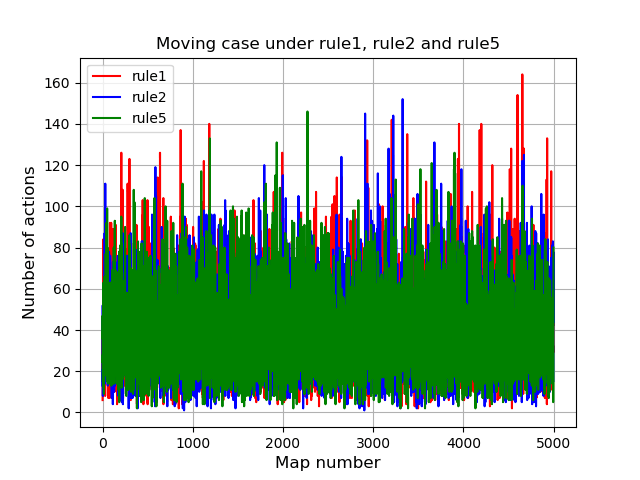
\includegraphics[width=0.7\textwidth]{fig/part2-first.png}
		\caption{Number of actions in moving case}
		\label{fig:part2-first}
	\end{figure}
	
	From the figure above, we find that the performance of 3 rules are similar, but Rule 1 has a minor disadvantage against Rule 2 and Rule 5. The means of Rule 1, Rule 2, and Rule 5 are 39.25, 37.82, and 38.04. The variances of Rule 1, Rule 2, and Rule 5 are 379.82, 347.52, and 351.06, from which we can see Rule 1 has a difference of ~3\% over the other two rules.
	

	In this problem, the target is moving and motion also counted as one step. We call this case ``moving and motion''. We use three rules to guide our search --- Rule 1, Rule 2, and Rule 5. Rule 1 and Rule 2 are just the original rules where motion is one step now. Rule 5 is designed for this specific problem. We generate 5000 maps and use these 3 rules to search the target in the maps. The result is shown in Fig \ref{fig:part2-last.png}.
	
	
	\begin{figure}[H]
		\centering
		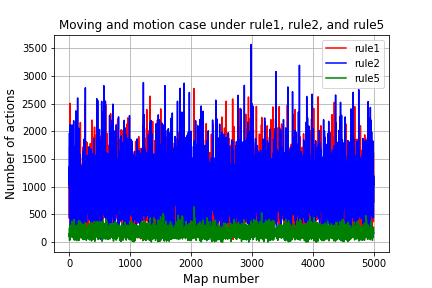
\includegraphics[width=0.7\textwidth]{fig/part2-last.png}
		\caption{Number of actions in moving and motion case}
		\label{fig:part2-last.png}
	\end{figure}
	
	From the figure above, it is easy to find that the performance of Rule 5 is better than Rule 1 and Rule 2. The means of Rule1, Rule 2, and Rule 5 are 938.88, 991.54, and 177.54.
	We can see that the average number of actions of Rule 5 is smaller than Rule 1 and Rule 2. The variances of Rule1, Rule 2, and Rule 5 are 154395.57, 176673.58, and 5534.82.
	From this view, we can also conclude that Rule 5 is better.
	
\end{document}